\section{Dati}
Gli ambiti più importanti nei quali vengono applicate tecniche di machine learning nella vita reale sono diversi, in particolare si usano in:
finanza, sanità, agricoltura, e-commerce, social, chatbot, sensoristica (come i veicoli a guida autonoma).
\\ Vista la grande mole di dati la necessità è quella di capire come trattare i dati.
\textbf{L'obiettivo del Machine Learning è sviluppare una metodologia per dare valore ai dati in funzione di una particolare domanda che ci stiamo ponendo.}

Tipicamente le tecniche di machine learning si dividono nelle seguenti tre macro categorie:
\begin{enumerate}
	\item \textit{Apprendimento supervisionato o predittivo:} qualcuno ha gia catalogato ad esempio delle immagini o dei dati e noi prendendo questi modelli dovremmo essere in grado di predire.
	\item \textit{Apprendimento non supervisionato o descrittivo:} ci sono delle funzioni obiettivo che vanno ottimizzate. Non usiamo etichette della singola istanza ma in qualche modo sappiamo dove arrivare.
	\item \textit{Apprendimento rinforzato:} E' quello più utile in questa epoca; il suo funzionamento è basato sui premi.
\end{enumerate}

In questo corso ci concentreremo sui primi due tipi di apprendimento.

L' \textit{apprendimento supervisionato} si divide a sua volta nelle seguenti due categorie:
\begin{itemize}
	\item Classificazione: quando il problema consiste nel dividere in classi delle quantità discrete.
	\item Regressione: quando il problema consiste nel ricostruire una certa variabile date delle condizioni pregresse.
\end{itemize}

L' \textit{apprendimento non supervisionato} si divide a sua volta in:
\begin{itemize}
	\item Clustering: Quando il problema consiste nel ricostruire delle classi delle istanze che ci vengono consegnate, senza sapere nulla sulla storia pregressa.
	\item Associativa: Quando il problema consiste nel scoprire pattern che descrivono bene caratteristiche associate ad un certo fenomeno.
\end{itemize}

Per alcuni compiti la correlazione statistica va benissimo, in alcuni casi però essa è addirittura deleteria.  Se infatti provassi a vedere la correlazione tra il numero di omicidi in America e il numero di fondi investiti sulla ricerca scientifica vedrei che statisticamente sono strettamente correlate. Questo è un no-sense ed è il classico esempio di \textit{correlazione spuria.}
A confermare questa visione in cui il modello per una certa trattazione dati è fondamentale è il famoso paradosso di Simpson. \\
\textbf{Paradosso di Simpson:} Utilizzare i dati senza un modello valido non porta alla scoperta della verità.


\subsection{Data types(*)}

Il primo passo fondamentale è quello di prendere confidenza coi dati. E' quindi molto importante capire la natura intrinseca dei dati che abbiamo a disposizione per risolvere in modo efficace un problema, in particolare, questi sono solitamente organizzati in strutture che chiamiamo \textbf{dataset}. Per le analisi con le tecniche di Machine Learning esse non sono altro che tabelle fatte da righe e da colonne.

\begin{defn}
	Definiamo \textbf{attributi} le colonne del dataset
\end{defn}
\begin{defn}
	Definiamo \textbf{istanze} le righe del dataset
\end{defn}

Ogni attributo è caratterizzato dal fatto di avere un \textit{tipo}, la sua conoscenza è fondamentale perché ci permette di sapere le proprietà che questo possiede.
In particolare, gli attributi si dividono in due grandi gruppi:
\begin{itemize}
	\item \textit{Categorici:}
	\begin{itemize}
		\item Nominali: ad esempio il colore degli occhi.
		\item Ordinali: ad esempio possono essere i giudizi.
	\end{itemize}
	\item \textit{Numerici:}
	\begin{itemize}
		\item Intervallo: ammettono operazioni di somma e sottrazione. 
		\item Ratio: possiamo applicare tutte le operazioni logico/matematiche.
	\end{itemize}
\end{itemize}


\begin{figure}[H]
	\centering
	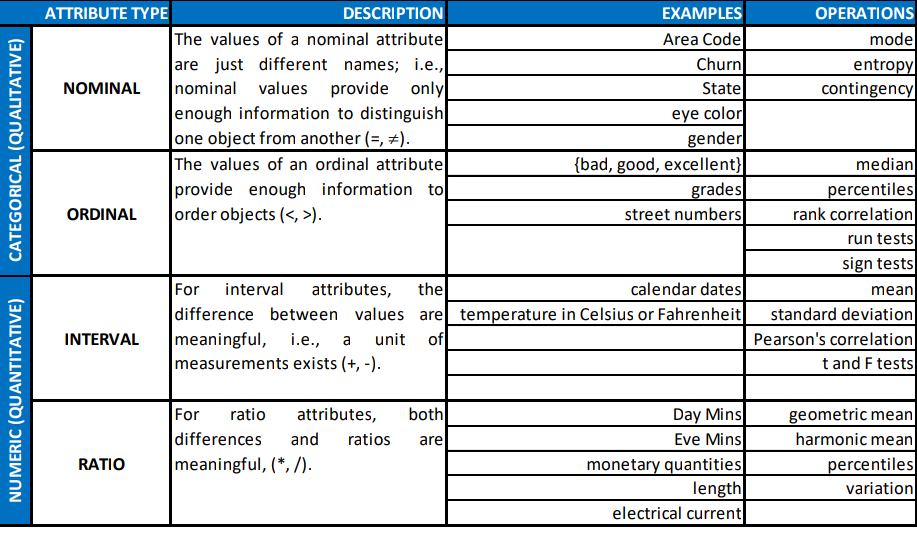
\includegraphics[height=0.5 \linewidth]{introduction/pict/attributi.png}
	\caption{Esempi di attributi divisi per categoria con le relative proprietà.}
\end{figure}
Dall'alto al basso il livello gerarchico sale e le proprietà aumentano.

C'è un'ulteriore divisione che può essere fatta ed è quella in:
\begin{itemize}
	\item Discreti (in cui la serie dei valori è finita o una infinità numerabile), che a loro volta si suddividono in:
	\begin{itemize}
		\item Categorici
		\item Numerici
		\item Binari: sono i più particolari da trattare, e hanno una serie di proprietà strane.
	\end{itemize}
	\item Continui: i cui valori sono numeri reali.
\end{itemize}

\subsection{Data exploration(*)}

E' utile sapere come esplorare i dati in modo intelligente usando tutti gli strumenti a disposizione. Di seguito un elenco degli strumenti statistici più utili che permettono di effettuare un'esplorazione completa dei dati.

\subsubsection{Definizioni}
\begin{defn}
	Si definisce \textbf{quantile} di ordine $\alpha$ il valore $q_{\alpha}$ che divide la popolazione in due parti proporzionali rispettivamente ad $\alpha$ e a $(1 - \alpha)$ e caratterizzate da valori rispettivamente minori e maggiori di $q_{\alpha}$
\end{defn}

Un quantile molto importante è il quantile di ordine $\frac{1}{2}$ che viene definito \textbf{mediana}, per come costruito questo è il valore che ha esattamente minori di lui  metà dei dati.

\begin{defn}
	Si definisce \textbf{media} il seguente valore:
	\[mean = \frac{1}{n}\sum_{i=1}^{n}x_i\]
\end{defn}


La media non è un buon modo di visualizzare i dati perché dice poco riguardo alla loro distribuzione. Essendo la media basata su singole osservazioni è fortemente soggetta a variazioni quando si hanno valori fortemente discostati dalla distribuzione dei dati.
Tali valori si chiamano \textit{outlier} e sono particolarmente interessanti da trattare.

Per ovviare a questo problema si è soliti usare  la \textbf{media trimmed} in cui si buttano via il valore più piccolo e il valore più grande. 
\begin{defn}
	Si definisce \textbf{media trimmed} il seguente valore:
	\[mean_{trimmed} = \frac{1}{n}\sum_{i=1}^{n}x_i  \qquad x_{i} = x - \max{x}- \min{x}\]
\end{defn}

Se si trova un grosso scostamento tra la media e la media trimmed probabilmente si ha la presenza di almeno un outlier.

\begin{defn}
	Si definisce \textbf{range} il seguente valore:
	\[ range = \max{x}- \min{x}\]
\end{defn}

Questo valore serve a quantificare la dispersione dei dati, ovviamente può essere fuorviante qualora i valori siano concentrati in una stretta banda. Per ovviare a questo problema si usa la varianza.

\begin{defn}
	Si definisce \textbf{varianza} il seguente valore:
	\[ var =  \sigma^{2} =\frac{1}{n - 1 }\sum_{i = 1}^{n} (x_{i} - \bar{x})^{2}\]	
\end{defn}

E' preferibile però usare la deviazione standard in quanto per come è definita risulta essere della stessa unità di misura dei dati.
\begin{defn}
	Si definisce \textbf{deviazione standard} il seguente valore:
	\[ std = \sigma =  \sqrt{\sigma^{2}} \]
\end{defn}

Essendo queste due grandezze definite a partire dalla media esse soffrono dello stesso problema: \textit{sono fortemente condizionate dagli outlier}; con lo stesso metodo precedente si definiscono, quindi, altre due grandezze in grado di ovviare a questo problema.

\begin{defn}
	Si definisce \textbf{deviazione media assoluta} il seguente valore:
	\[ AAD =  \frac{1}{n}\sum_{i=1}^{n}|x_i- mean|\]
\end{defn}

\begin{defn}
	Si definisce \textbf{deviazione mediana assoluta} il seguente valore:
	\[ MAD = mediana(x_{1}-mean, x_{2}-mean, ..., x_{n0}-mean )\]
\end{defn}

E' utile anche definire il range interquartile (IQR) per le stesse ragioni precedenti.

\begin{defn}
	Si definisce \textbf{Range InterQuartile} il seguente valore:
	\[ IQR = q_{75\%} - q_{25\%}\]
\end{defn}

Ci sono anche diverse grandezze utili da definire nei casi in cui si ha a che fare con coppie di attributi, in tal caso:

\begin{defn}
	Si definisce \textbf{covarianza} il seguente valore:
\[cov(X,Y) = \frac{1}{m -1}\sum_{i = 1}^{m} (x_{i} - \bar{x})(y_{i} - \bar{y})\]
\end{defn}

Per come è costruita questa matrice è necessariamente quadrata, e il suo valore $ij$-esimo rappresenta la covarianza tra il valore $i$-esimo dell'attributo x e il valore $j$-esimo dell'attributo y.

Un'ulteriore misura dell'associazione tra le coppie di attributi quantitativi che non dipende dalla varianza di ciascun attributo è la seguente:

\begin{defn}
	Si definisce \textbf{correlazione di Pearson} il seguente valore:
	\[ corr(x,y) = \frac{cov(x,y)}{\sqrt{var(x)var(y)}}\]
\end{defn} 
Per come è definita si ha ovviamente che: $cov(x,y) \in [-1,1]$.

\subsubsection{Visualization}
E' molto utile visualizzare i dati quando bisogna lavorarci, questo fondamentalmente per due motivi:
\begin{itemize}
	\item Ci permette di trovare pattern tra le variabili che valori puntuali non ci permetterebbero di trovare.
	\item Ci permette di visualizzare i risultati di una lavorazione fatta sui dati.
\end{itemize}

Di seguito proponiamo un rapido elenco dei grafici più utili e descriviamone le varie caratteristiche.

I dati possono essere organizzati in istogrammi caratterizzati dalla presenza di bin(indicano la larghezza in cui i dati sono organizzati). A seconda dell'ampiezza che uso posso ottenere due disegni molto diversi come mostrato in figura.


\begin{figure}[H]
	\centering
	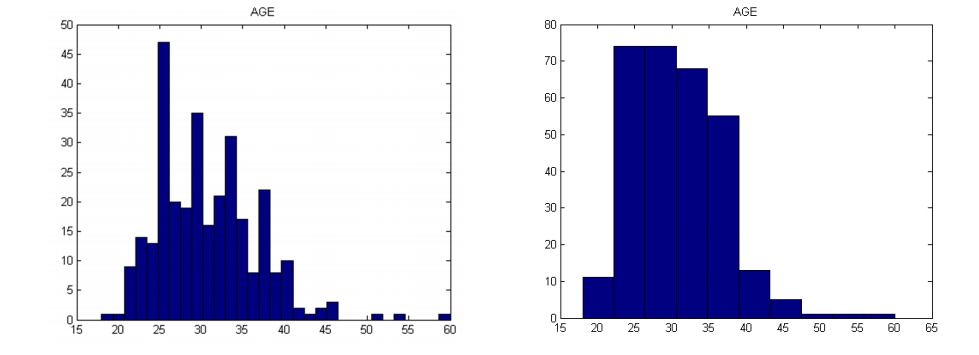
\includegraphics[height=0.35 \linewidth]{introduction/pict/istogramma_quant.png}
	\caption{Differenza tra due istogrammi fatti sulla stessa distribuzione di dati ma con numero di bin diversi.}
\end{figure}


Si possono allo stesso modo creare istogrammi per dati qualitativi. La differenza rispetto agli istogrammi sui dati quantitativi è quella per cui ogni bin corrisponde ad una categoria diversa.

\begin{figure}[H]
	\centering
	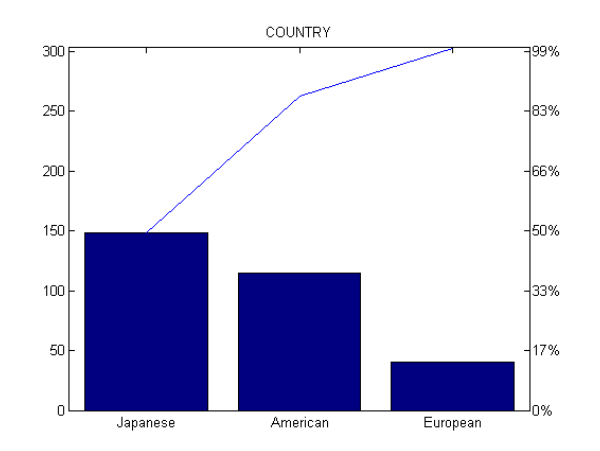
\includegraphics[height=0.3 \linewidth]{introduction/pict/istogramma_qual.png}
	\caption{Istogramma fatto su  dati qualitativi.}
\end{figure}

In questo caso la linea blu disegnata sopra è una linea cumulativa, ossia rappresenta dove si trova il livello sommando tutti i dati che man mano incontro, per come è costruita ovviamente dovrà finire sul valore $100\%$


Un altro modo di rappresentare i dati particolarmente utile è il \textbf{grafico Box and Whiskers} applicato solo ad attributi quantitativi. Rispetto agli istogrammi questo è decisamente più utilizzato perché permette di estrarre  più informazioni. In particolare, proponiamo un grafico in cui sono esplicitate le informazioni ottenibili:

\begin{figure}[H]
	\centering
	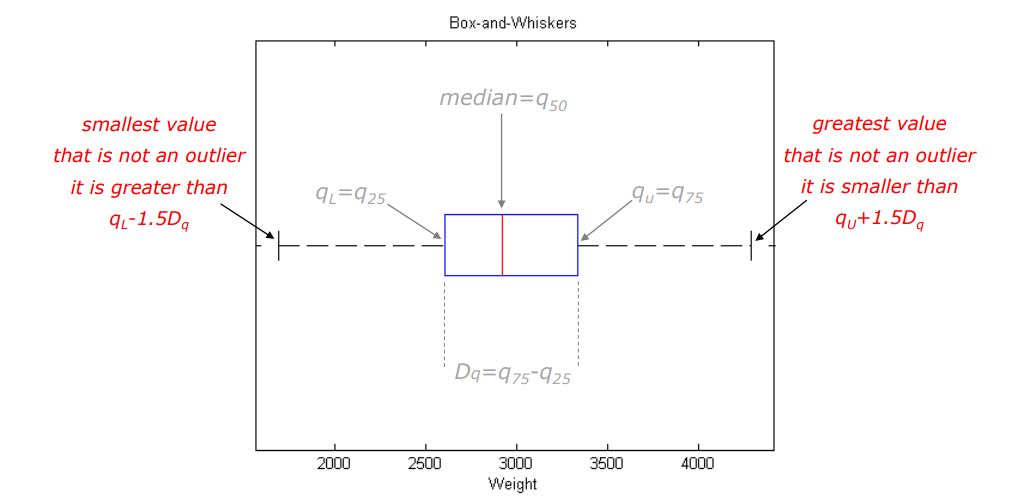
\includegraphics[height=0.4 \linewidth]{introduction/pict/box_plot.png}
	\caption{Informazioni ottenibili da un box plot.}
\end{figure}


\subsection{Missing replacement(*)}

E' la parte dell'analisi dati che si occupa di studiare come sostituire i valori mancanti di certi attributi in un dataset. Essendo un problema di così larga portata possiamo capire bene che una trattazione esaustiva riempirebbe le ore di un intero corso, tuttavia ne forniamo le basi per essere in grado di poter effettuare una analisi dati efficace. 

Le motivazioni principali del perché un database presenta delle mancanze sono le seguenti:
\begin{itemize}
	\item Tale valore non è stato possibile misurarlo.
	\item Non si conosce con esattezza tale valore.
	\item Si è verificato qualche errore durante la presa dati.
	\item Quel determinato attributo fino ad un certo punto dell'analisi non è mai stato considerato importante e quindi non è mai stato registrato.
\end{itemize}

Ci sono diversi metodi che ci permettono di riempire quel valore mancante, di seguito diamo una rapida trattazione dei più usati:

\begin{itemize}
	\item \textbf{Record removal:} è il metodo più drastico e consistere nell'eliminare tutta l'istanza che contiene quel valore. Non viene usato frequentemente perché si rischia di perdere valori che possono essere fondamentali per l'analisi dati. \\ \textit{In particolare se la probabilità che un attributo abbia un valore nullo è: p(NULL) ed è un record con $m$ attributi allora la probabilità di non avere dati nulli in quel record diventa: 
		\[(1-p(NULL))^m\]}
	
	\item \textbf{Global constant:} consiste nel sostituire tutti i missing values con un valore costante chiamato \textit{place holder.} Tale metodo non è molto efficiente perché un valore costante non può essere rappresentativo di una distribuzione.
	
	\item \textbf{Manual imputation:} consiste nel sostituire manualmente i missing values tramite delle osservazioni. Lo svantaggio è che è tremendamente svantaggioso dal punto di vista computazionale.
	\item  \textbf{Moda replacement:} consiste nel rimpiazzare tutti i missing values con la moda di quel dato attributo, valgono le stesse considerazioni fatte per il metodo della global constant. Qualora gli attributi fossero continui si effettuerebbe la stessa cosa ma sostituendo la media.
	\item \textbf{Conditional mean replacement:} consiste nel rimpiazzare tutti i missing values con la media a condizione del fatto che sia presente un'ulteriore condizione posta su un secondo attributo. E' un po' più efficace degli altri elementi ma presenta anch'esso delle criticità.
	
	\item \textbf{Most probable:} consiste nell'eseguire una regressione sul nostro dataset utilizzando un altro attributo. In questo caso è possibile usare dei modelli di regressione anche molto complessi ed è possibile lavorare anche con dati qualitativi.
\end{itemize}

E' ora chiaro che il confine tra l'esplorazione dati e la modellizzazione degli stessi è molto sottile.

\subsection{Data Preprocessing(*)}

Il preprocessing è una fase dell'analisi dati che consiste nel \textbf{rendere i dati più fruibili per una analisi dati.} Elenchiamo di seguito le tecniche più utilizzate nella data preprocessing.

\subsubsection{Aggregation}
\textit{L'aggregazione consiste nel combinare due o più record in un unico oggetto.}
Ci sono diversi vantaggi ottenibili nell'aggregare i dati, in particolare:

\begin{itemize}
	\item \textit{Dataset più piccoli:} durante un'analisi dati abbiamo bisogno di usare il minor quantitativo di memoria e di tempo; l'aggregazione diminuisce il tempo di esecuzione di un algoritmo.
	\item \textit{Cambiamento di scopo:} ci permette di avere una visione più ampia dei dati qualora cambiassimo lo scopo della nostra analisi in corso d'opera.
	\item \textit{Varianza ridotta:} gli attributi calcolati su record aggregati sono più stabili rispetto a quelli associati ai record nativi, questo per un effetto statistico.
\end{itemize}


\subsubsection{Sampling}
In molti casi avere una quantità enorme di dati può essere deleterio dal punto di vista computazionale, questo perché bisognerebbe usare algoritmi più semplificati in modo che la computazione possa essere svolta su un maggior numero di dati. Ciò che dobbiamo preferire è invece usare un algoritmo migliore su un dataset ridotto. Per questo entra in gioco il concetto di \textbf{campionamento.}

Il problema si traduce nella seguente domanda: \textit{quando un campione è rappresentativo?}

\begin{defn}
	Un campione si dice \textbf{rappresentativo} quando ha approssimativamente le stesse proprietà del dataset di partenza.
\end{defn}

Dobbiamo quindi trovare uno schema che ci permetta di scegliere \textit{con grande probabilità} dei campioni rappresentativi. In questo caso il problema si riduce a trovare le appropriate:
\begin{itemize}
	\item Dimensioni del campione.
	\item Tecniche di campionamento.
\end{itemize}
Esistono moltissime tecniche di campionamento e di seguito  mostriamo le più basilari:

\begin{itemize}
	\item \textbf{Simple Random Sampling:} Ogni record del dataset ha la stessa probabilità di essere incluso nel campione. Tale record può essere rimosso o meno dal dataset di partenza. Quando i campioni sono molto piccoli rispetto al dataset di partenza la rimozione o meno genera due campioni che sono molto simili.	
	Questo metodo fallisce quando il datset consiste di attributi qualitativi in modo che i possibili valori che possono avere hanno frequenze fortemente diverse.
	
	\item \textbf{Stratified Sampling:} Vengono presi record in modo che all'interno del campione vengano rispettate le proporzioni tra gli attributi presenti nel dataset di partenza.
\end{itemize}

Una volta scelta la tecnica di campionamento dobbiamo occuparci di scegliere la grandezza del campione. Tenere un campione di grande ampiezza aumenta la probabilità che un campione sia rappresentativo, di contro elimina la maggior parte dei vantaggi computazionali di avere un campionamento. Avere un campione troppo piccolo invece manda in contro al rischio di eliminare pattern potenzialmente importanti o addirittura di mantenere pattern erronei. La giusta dimensione del campionamento va scelta in base al nostro dataset di riferimento effettuando delle prove.

\subsubsection{Dimensionality reduction}

In diversi casi capiterà di dover analizzare dataset caratterizzati da un gran numero di attributi. Diminuirne il numero porta a diversi vantaggi:

\begin{itemize}
	\item Molti algoritmi lavorano meglio se la dimensionalità è minore.
	\item L'interpretabilità del modello implementato aumenta perché dipende da un numero minore di attributi.
	\item La rappresentazione grafica dei dati è facilitata.
	\item L'ammontare di tempo e memoria diminuisce drasticamente.
\end{itemize}

Contrariamente a ciò che ci si aspetterebbe \textit{avere una dimensionalità maggiore dei dati non implica un aumento delle performance.}
Mostriamo questo dato con il sgeuente grafico.

\begin{figure}[H]
	\centering
	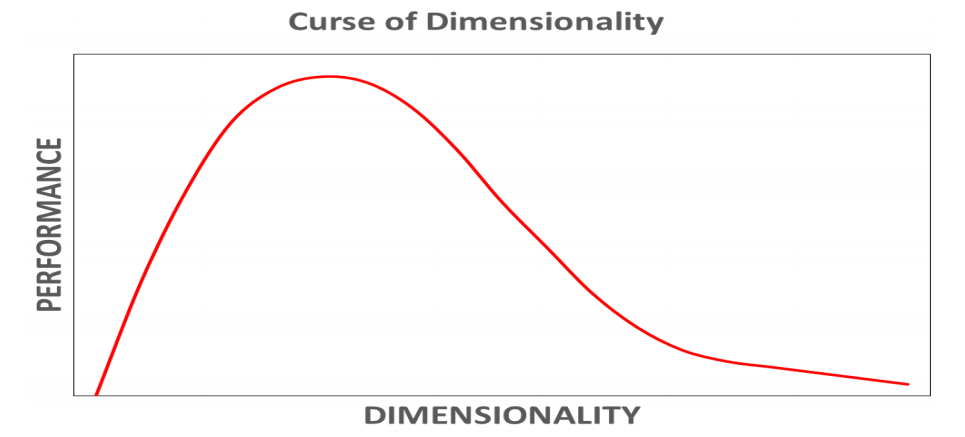
\includegraphics[height=0.35 \linewidth]{introduction/pict/performance.png}
	\caption{Andamento delle performance di un algoritmo in funzione della dimensionalità del dataset.}
\end{figure}

Molte delle tecniche usate per ridurre le dimensionalità sfruttano tecniche prese dall'algebra lineare per proiettare i dati da uno spazio dimensionale maggiore ad uno spazio dimensionale minore.

La \textbf{Principal Component Analysis (PCA)} trova nuovi attributi in modo che:
\begin{itemize}
	\item Siano \textit{combinazione lineari} degli attributi di partenza.
	\item Siano \textit{mutualmente ortogonali.}
	\item Catturino il \textit{massimo ammontare di variabilità} nei dati.
\end{itemize}

In particolare la \textbf{Singular Value Decomposition (SVD)} è una tecnica di algebra lineare correlata alla PCA ed è largamente usata per ridurre la dimensionalità dei dataset.

\begin{defn}
	Si definisce \textbf{binarizzazione} la tecnica di trasformazione di attributi continui e categorici in uno o più attributi binari.
\end{defn}
Per binarizzare un attributo si associano $k$ possibili valori a $k$ valori interi nell'intervallo $[0, k-1]$. Successivamente si trasformano questi k interi in un numero binario; come è noto il numero di cifre necessarie per rappresentare un numero intero son le seguenti:
\[s = \lfloor \log_{2}k \rfloor\] 
 In questo caso è necessario introdurre un attributo binario per ogni attributo categorico con cui il dato può manifestarsi. Ovviamente si è più interessati ai casi in cui si manifesta il valore 1 perché indica la presenza di tale attributo.

 Quando, invece, si ha a che fare con attributi durante un'analisi di classificazione o di associazione bisogna ricorrere alla tecnica di \textbf{discretizzazione.} Come facilmente intuibile la miglior discretizzazione dipende dal tipo di algoritmo che sto utilizzando.
 La discretizzazione può essere:
 
 \begin{itemize}
 	\item \textbf{Supervisionata.}
 	\item \textbf{Non-supervisionata.}
 \end{itemize}
La \textit{discritezzizazione supervisionata} utilizza ulteriori informazioni (attributi di classe) per discretizzare gli attributi. Questa tecnica divide i punti in modo che qualche misura di \textit{purità} sia massimizzata. La misura di purità più spesso applicata è l'\textbf{entropia.}
 	
 	\[e_{i} = - \sum_{k = 1}^{K}p_{ki}\log_{2}p_{ki}\]
 	
Per come è costruita si ha che:
\begin{itemize}
	\item Se contiene solo record di una data classe $\implies e_{i} = 0$, massima purità. 
	\item Se contiene egualmente spesso tutte le class $\implies e_{i} = \max$, minima purità. 
\end{itemize}

La discretizzazione supervisionata basata sull'entropia permette di trovare i punti di divisione degli attributi \textit{continui} tali che l'entropia totale sia \textit{minimizzata.}

\begin{defn}
	Si definisce entropia totale la seguente espressione:
	\[ E = \sum_{i = 1}^{n}w_{i}e_{i}\] 
	In cui:
	\[w_{i} = \frac{m_{i}}{m}\]
	E le variabili sono così definite: \begin{itemize}
		\item $n$: numero di intervalli.
		\item $m$: numero di record.
		\item $m_{i}$: numero di record nell'intervallo i-esimo.
	\end{itemize}
\end{defn}


 	
La \textit{discretizzazione non-supervisionata} non utilizza alcuna informazione eccetto il valore dell'attributo continuo da discretizzare. Possono essere a loro volta divisi in due categorie:
 	\begin{itemize}
 		\item \textbf{Equal width unsupervised discretization:}  gli intervalli in cui viene discretizzato hanno tutti la stessa ampiezza.
 		\item  \textbf{Equal frequency unsupervised discretization:} gli intervalli in cui viene discretizzato hanno approssimativamente la stessa frequenza.
 	\end{itemize}
 
 
 Può succedere però che gli attributi categorici abbiano troppi valori. Se gli attributi  in questione sono ordinali allora si applicano le tecniche viste in precedenza, se invece sono nominali allora bisogna trovare un altro approccio. In questo caso possiamo infatti raggruppare i valori solo se il raggruppamento si traduce in un miglioramento nelle performance di classificazione o nel raggiungimento di qualche obiettivo del trattamento dati. 
\subsubsection{Variable transformation}

\begin{defn}
Si definisce \textbf{trasformazione di variabile} qualsiasi trasformazione applicata a tutti i valori di quella variabile.
\end{defn}

Ci sono due tipi di trasformazione di variabile:
\begin{itemize}
	\item \textbf{Funzioni semplici}: una semplice funzione matematica è applicata a tutti i valori di una variabile individualmente. Bisogna stare attenti all'ordine in cui vengono applicate e soprattutto a come si comporta la funzione per valori negativi e vicini allo 0.
	\item \textbf{Standardizzazione:} trasforma tutto il dataset in modo che acquisiscano una particolare proprietà.
	\[Z = \frac{x - \mu}{\sigma}\]
	E' molto importante perché il nuovo dataset viene trasformato in modo da avere $\mu = 0$ e $\sigma = 1$. In questo modo la somma di diversi attributi continui permette ad uno o a pochi attributi di prendere grandi valori e di dominare il nuovo attributo somma. E' molto utile quindi perché fa saltare immediatamente all'occhio la presenza di outlier.
	
	In questo caso la media è sostituita dalla mediana, e la deviazione standard è sostituita dalla AAD che ricordiamo essere definita come:
	\[\sigma_{x} = \frac{1}{m} \sum_{i = 1}^{m}|x_{i}- \mu|\]
\end{itemize}
